\documentclass[a4paper]{article}
\usepackage{lmodern}
\usepackage{amssymb,amsmath}
\usepackage{ifxetex,ifluatex}
\usepackage{fixltx2e} % provides \textsubscript
\ifnum 0\ifxetex 1\fi\ifluatex 1\fi=0 % if pdftex
  \usepackage[T1]{fontenc}
  \usepackage[utf8]{inputenc}
\else % if luatex or xelatex
  \ifxetex
    \usepackage{mathspec}
  \else
    \usepackage{fontspec}
  \fi
  \defaultfontfeatures{Ligatures=TeX,Scale=MatchLowercase}
\fi
% use upquote if available, for straight quotes in verbatim environments
\IfFileExists{upquote.sty}{\usepackage{upquote}}{}
% use microtype if available
\IfFileExists{microtype.sty}{%
\usepackage{microtype}
\UseMicrotypeSet[protrusion]{basicmath} % disable protrusion for tt fonts
}{}
\usepackage[margin=1in]{geometry}
\usepackage{hyperref}
\hypersetup{unicode=true,
            pdftitle={Avaliação pela Moda, Média ou Mediana?},
            pdfauthor={Luiz Fernando Palin Droubi; Norberto Hochheim; Willian Zonato},
            pdfborder={0 0 0},
            breaklinks=true}
\urlstyle{same}  % don't use monospace font for urls
\usepackage{graphicx,grffile}
\makeatletter
\def\maxwidth{\ifdim\Gin@nat@width>\linewidth\linewidth\else\Gin@nat@width\fi}
\def\maxheight{\ifdim\Gin@nat@height>\textheight\textheight\else\Gin@nat@height\fi}
\makeatother
% Scale images if necessary, so that they will not overflow the page
% margins by default, and it is still possible to overwrite the defaults
% using explicit options in \includegraphics[width, height, ...]{}
\setkeys{Gin}{width=\maxwidth,height=\maxheight,keepaspectratio}
\IfFileExists{parskip.sty}{%
\usepackage{parskip}
}{% else
\setlength{\parindent}{0pt}
\setlength{\parskip}{6pt plus 2pt minus 1pt}
}
\setlength{\emergencystretch}{3em}  % prevent overfull lines
\providecommand{\tightlist}{%
  \setlength{\itemsep}{0pt}\setlength{\parskip}{0pt}}
\setcounter{secnumdepth}{5}
% Redefines (sub)paragraphs to behave more like sections
\ifx\paragraph\undefined\else
\let\oldparagraph\paragraph
\renewcommand{\paragraph}[1]{\oldparagraph{#1}\mbox{}}
\fi
\ifx\subparagraph\undefined\else
\let\oldsubparagraph\subparagraph
\renewcommand{\subparagraph}[1]{\oldsubparagraph{#1}\mbox{}}
\fi

%%% Use protect on footnotes to avoid problems with footnotes in titles
\let\rmarkdownfootnote\footnote%
\def\footnote{\protect\rmarkdownfootnote}

%%% Change title format to be more compact
\usepackage{titling}

% Create subtitle command for use in maketitle
\newcommand{\subtitle}[1]{
  \posttitle{
    \begin{center}\large#1\end{center}
    }
}

\setlength{\droptitle}{-2em}
  \title{Avaliação pela Moda, Média ou Mediana?}
  \pretitle{\vspace{\droptitle}\centering\huge}
  \posttitle{\par}
\subtitle{Teoria e simulações}
  \author{Luiz Fernando Palin Droubi\footnote{SPU/SC,
  \href{mailto:luiz.droubi@planejamento.gov.br}{\nolinkurl{luiz.droubi@planejamento.gov.br}}} \\ Norberto Hochheim\footnote{UFSC,
  \href{mailto:hochheim@gmail.com}{\nolinkurl{hochheim@gmail.com}}} \\ Willian Zonato\footnote{SPU/SC,
  \href{mailto:willian.zonato@planejamento.gov.br}{\nolinkurl{willian.zonato@planejamento.gov.br}}}}
  \preauthor{\centering\large\emph}
  \postauthor{\par}
  \predate{\centering\large\emph}
  \postdate{\par}
  \date{25/05/2018}

\usepackage[brazil]{babel}
\usepackage{graphicx}
\usepackage{float}
\usepackage{subfig}
\usepackage{caption}
\newcommand{\pkg}[1]{{\normalfont\fontseries{b}\selectfont #1}}
\let\proglang=\textsf
\let\code=\texttt
\usepackage{booktabs}
\usepackage{longtable}
\usepackage{array}
\usepackage{multirow}
\usepackage[table]{xcolor}
\usepackage{wrapfig}
\usepackage{float}
\usepackage{colortbl}
\usepackage{pdflscape}
\usepackage{tabu}
\usepackage{threeparttable}
\usepackage[normalem]{ulem}

\begin{document}
\maketitle

``Eu sou o homem que com a máxima ousadia descobriu o que já fora
descoberto antes.'' (CHESTERTON,
\protect\hyperlink{ref-gkchesterton}{2008}, p. 12).

\section{INTRODUÇÃO}\label{introducao}

Existe na área da avaliação de imóveis uma discussão frequente e
indesejável a respeito da adoção da estimativa de tendência central
adotada para a predição de valores quando da utilização de modelos
lineares log-normais, isto é, modelos em que a variável resposta aparece
transformada pela função logaritmo natural.\footnote{Neste artigo esta
  função é representada por \(log\).}

Pretende-se com este artigo dar a este problema de uma abordagem formal.
Entendemos que a norma brasileira (ABNT,
\protect\hyperlink{ref-NBR1465302}{2011}) deveria tratar este assunto de
maneira clara, especificando qual estimador deveria ser utilizado para a
formação de valores, dependendo do método utilizado.

\begin{quote}
Major Point 1: When we talk about the relationship of one variable to
one or more others, we are referring to the regression function, which
expresses the mean of the first variable as a function of the others.
The key word here is \emph{mean}! (MATLOFF,
\protect\hyperlink{ref-matloff2009}{2009}, p. 386, grifo do autor)
\end{quote}

Tem que se levar em conta que a equação de regressão linear não é uma
equação determinística, mas probabilística. No dia-a-dia da prática de
engenharia de avaliações, assim como em outras áreas, no entanto, a
equação de regressão é usualmente escrita simplificadamente, sem o termo
de erro \(\epsilon\), ou seja, a equação de regressão é escrita como uma
equação determinística, da forma:

\[Y = \alpha + X\beta\] A equação acima é uma simplificação da equação
de regressão, haja vista que ela presume que as hipóteses clássicas da
regressão linear são atendidas, entre elas, a hipótese que os erros são
normais e tem média zero (\(\epsilon \sim N(0, \sigma^2)\)).

Num modelo onde não há a adoção de qualquer transformação para a
variável dependente, verificada a hipótese da normalidade, esta equação
de regressão é também a equação de estimação da variável \(Y\), ou seja,
para uma equação de regressão sem transformação de variáveis, pode-se
escrever:

\[E[Y|X] = E[\alpha + X\beta] + E[\epsilon] = \alpha + X\beta\] Haja
vista que o valor esperado para o termo de erro \(\epsilon\) é zero.

No entanto, quando a variável dependente \(Y\) é transformada, este
termo de erro desprezado na equação de regressão acima é de suma
importância para o computo do valor esperado da variável original, como
veremos neste artigo, pois ele determina a equação de estimação da
variável original. Por exemplo, no caso que aqui nos interessa, que é o
da transformação logarítmica da variável dependente, temos:

\[log(Y) = \alpha + X\beta + \epsilon \Leftrightarrow\]
\[Y = \exp(\alpha + X\beta)\exp(\epsilon) \Leftrightarrow\]
\[E[Y|X] = E[\exp(\alpha + X\beta)]E[\exp(\epsilon)|X] \Leftrightarrow\]
\[E[Y|X] = \exp(\alpha + X\beta)E[\exp(\epsilon)|X]\]

O fundamental a se perceber aqui é que, quando há transformação da
variável dependente, para voltarmos à variável original, temos que levar
em conta o termo de erro, haja vista que uma propriedade do valor
esperado é a de que \(E[f(X)] \ne f(E[X])\), como veremos a seguir. Mais
precisamente, para funções convexas, pela desigualdade de Jensen,
\(f(E[X]) \leq E[(f(x)]\). Isto implica que o valor esperado da
exponencial do termo de erro que precisamos estimar é maior do que a
exponencial do valor esperado do erro, ou seja,
\(E[\exp(\epsilon)|X] \geq \exp(E[\epsilon|X]) = 1\).

\section{REVISÃO BIBLIOGRÁFICA}\label{revisao-bibliografica}

\subsection{A avaliação pela moda}\label{a-avaliacao-pela-moda}

GIANNAKOS; LEÃO (\protect\hyperlink{ref-giannakos}{1996}) faz uma
crítica à avaliação pela moda da distribuição lognormal, crítica esta
muito bem elaborada e da qual não discordamos no todo. Porém, o mesmo
trabalho faz também uma defesa a nosso ver injustificada da utilização
da estimativa pela mediana desta distribuição. Concordamos com
GIANNAKOS; LEÃO (\protect\hyperlink{ref-giannakos}{1996}) que a moda não
é o valor mais provável, contudo, a nosso ver, pelo motivo que \textbf{o
valor mais provável é o Valor Esperado} da variável, ou seja, o seu
valor médio, como veremos.

Mesmo em GIANNAKOS; LEÃO (\protect\hyperlink{ref-giannakos}{1996}),
encontra-se que ``a média aritmética é o `valor esperado' da variável''.
No entanto, a nosso ver GIANNAKOS; LEÃO
(\protect\hyperlink{ref-giannakos}{1996}) não analisou apropriadamente
este valor esperado e suas propriedades, assim como determiná-lo
apropriadamente no caso da transformação de variáveis em modelos de
regressão linear.

Segundo Giannakos e Leão (\protect\hyperlink{ref-giannakos}{1996}, p.
5), a média:

\begin{quote}
introduz, na regressão linear, como fator de decisão, as características
da função dita ``originária'', não-linear, transformada em logarítmica
precisamente para alcançar linearidade; viola os pressupostos do método
de mínimos quadrados, fundamento da regressão, ou, alternativamente,
equivale a adulterar a amostra original, multiplicando, no caso
presente, todos os seus valores por 1,04968. Além disto, substitui,
arbitrariamente, o componente aleatório da avaliação por valor
determinado, que distorce o resultado visado. Finalmente, onde a moda
subestima o valor dos quocientes Y/Yc, a média o superestima, embora em
escala menos pronunciada. Aliás, nunca é demais repetir, a razão
principal para rejeitar toda e qualquer tentativa de avaliar seja ``pela
Moda'', ``pela Média'' ou ``pela Mediana'' está na interpretação
implícita, de que se estaria avaliando a variável Y ou os quocientes
Y/Yc, quando, na realidade, está-se lidando tão somente com a variável W
(ver equação 1), sem qualquer preocupação com sua origem ou
``paternidade''.
\end{quote}

Pretendemos demonstrar com este artigo que esta abordagem está
equivocada e que, à partir do modelo de regressão linear obtido pelo
métodos dos mínimos quadrados, a estimativa adequada seria a justamente
a estimava pela média da distribuição, como veremos a seguir.

\subsection{Esperança matemática ou Valor
Esperado}\label{esperanca-matematica-ou-valor-esperado}

Segundo BENNETT (\protect\hyperlink{ref-bennett}{2006}), a
\textbf{esperança matemática} ou \textbf{valor esperado } de uma
variável aleatória é a soma do produto de cada probabilidade de saída da
experiência pelo seu respectivo valor. Isto é, representa o valor médio
`esperado' de uma experiência se ela for repetida muitas vezes.
Matematicamente, a Esperança de uma variável aleatória \(X\) é
representada pelo símbolo \(E(X)\), de tal forma que, pela definição
dada acima, no caso de uma variável aleatória discreta:

\[E(X) = \sum_{i = 1}^{\infty}x_ip(x_i)\]

Já para uma variável aleatória contínua \(x\), o valor esperado ou o
valor médio de \(x\) torna-se:

\[E(X) = \int_{-\infty}^{\infty}xf_Y(x)dx\]

onde \(f_Y(x)\) é a função densidade de probabilidade de \(x\).

\subsubsection{Propriedades}\label{propriedades}

Sejam \(a\) e \(b\) dois escalares (BENNETT,
\protect\hyperlink{ref-bennett}{2006}, p. 6):

\(E(aX + b) = aE(X) + b\) e \(E[az(X) + b] = aE[z(X)] + b.\)

Seja \(X\) e \(Y\) duas variáveis aleatórias independentes \(X\) e
\(Y\), então:

\(E(XY) = E(X)E(Y)\)

Porém, se \(X\) e \(Y\) não forem independentes, esta propriedade falha
(covariância).

\subsubsection{Desigualdade de Jensen}\label{desigualdade-de-jensen}

Segundo , seja \(\varphi(x)\) uma função convexa, então:

\(\varphi \left(\operatorname {E} [X]\right)\leq \operatorname {E} \left[\varphi (X)\right].\)

Como pode-se demonstrar, a função \(e^x\) é uma função convexa, pois
possui derivada segunda sempre maior que zero (\({f}''=e^x>0\)).

\subsection{Estimadores}\label{estimadores}

\begin{quote}
Earlier, we often referred to certain estimators as being ``natural.''
For example, if we are estimating a population mean, an obvious choice
of estimator would be the sample mean. But in many applications, it is
less clear what a ``natural'' estimate for a population quantity of
interest would be. We will present general methods for estimation in
this section. We will also discuss advanced methods of inference
(MATLOFF, \protect\hyperlink{ref-matloff2009}{2009}, p. 303).
\end{quote}

A definição de um \emph{estimador} para um parâmetro ou uma variável
\(\theta\) é uma função \(\hat{\theta}(X)\), que mapeia o espaço
amostral para um conjunto de estimativas amostrais, em que \(X\) é uma
variável aleatória dos dados observados. É usual denotar uma estimativa
em para um determinado ponto \(x \in X\) por \(\hat{\theta}(X = x)\) ou,
mais simplesmente, \(\hat{\theta}(x)\).

\subsubsection{Propriedades de um
estimador}\label{propriedades-de-um-estimador}

\paragraph{Erro}\label{erro}

\[e(x) = \hat{\theta}(x) - \theta\]

\paragraph{Desvio}\label{desvio}

\[d(x) = \hat{\theta}(x) - E(\hat{\theta}(X))\] onde
\(E(\hat{\theta}(X))\) é o Valor Esperado do estimador.

\paragraph{Variância}\label{variancia}

\[\text{Var}(\hat{\theta}) = E[(\hat{\theta} - E(\hat{\theta})^2]\]

\paragraph{Viés}\label{vies}

\[B(\hat{\theta}) = E(\hat{\theta}) - \theta\]

O viés coincide com o valor esperado do erro, pois
\(E(\hat{\theta}) - \theta = E(\hat{\theta}-\theta)\).

Numa regressão linear:

\[B[\hat{\mu}(x_0)] = E[\hat{\mu}(x_0)] - \mu(x_0)\]

\paragraph{Erro médio quadrático}\label{erro-medio-quadratico}

Segundo Shen e Zhu (\protect\hyperlink{ref-shen}{2008}, p. 553), o erro
médio quadrático é uma medida comum da qualidade de um estimador na
literatura estatística.

\[MSE = E[\hat{\theta}(X) - \theta]\]

Numa regressão linear, o erro médio quadrático pode ser descrito por:

\[MSE[\hat{\mu}(x_0)] = E[\hat{\mu}(x_0) - \mu(x_0)]^2 = \text{Var}[\hat{\mu}(x_0)] + \text{B}^2[\hat{\mu}(x_0)]\]

\paragraph{Consistência}\label{consistencia}

\[\lim_{n \rightarrow \infty}\hat{\theta} = \theta\]

\subsubsection{Melhor estimador linear não-inviesado ou
BLUE}\label{melhor-estimador-linear-nao-inviesado-ou-blue}

Em estatística, é comum o uso da sigla BLUE (\emph{Best Linear Unbiased
Estimator}) para indicar o melhor estimador linear não-enviesado.

\subsubsection{Tradeoff entre viés e
variância}\label{tradeoff-entre-vies-e-variancia}

\hypertarget{regressao-linear}{\subsection{Regressão
Linear}\label{regressao-linear}}

\subsubsection{Definição precisa}\label{definicao-precisa}

Sejam Y e X duas variáveis e \(m_{Y;X}(t)\) uma função tal que:

\[m_{Y;X}(t) = E(Y|X = t)\]

Chamamos \(m_{Y;X}\) de \textbf{função de regressão de \(Y\) dado \(X\)}
(MATLOFF, \protect\hyperlink{ref-matloff2009}{2009}, p. 386, grifo do
autor). Em geral, \(m_{Y;X}(t)\) é a \textbf{média} de \(Y\) para todas
as unidades da população para as quais \(X = t\) (MATLOFF,
\protect\hyperlink{ref-matloff2009}{2009}, p. 386, grifo nosso).

\begin{quote}
The word ``regression'' is an allusion to the famous comment of Sir
Francis Galton in the late 1800s regarding ``regression toward the
mean.'' This referred to the fact that tall parents tend to have
children who are less tall closer to the mean -- with a similar
statement for short parents. The predictor variable here might be, say,
the father's height F, with the response variable being, say, the son's
height S. Galton was saying that \(E(S|F) < F\).
\end{quote}

Segundo Matloff (\protect\hyperlink{ref-matloff2009}{2009}, p. 386,
grifo do autor), ainda, a função \(m_{Y;X}(t)\) é uma função da
\textbf{população}, ou seja, apenas \textbf{estimamos} uma equação de
regressão (\(\hat{m}_{Y;X}(t)\)) à partir de uma amostra da população.

\begin{quote}
The function \(m_{Y;X}(t)\) is a population entity, so we must estimate
it from our sample data. To do this, we have a choice of either assuming
that \(m_{Y;X}(t)\) takes on some parametric form, or making no such
assumption. If we opt for a parametric approach, the most common model
is linear {[}\ldots{}{]} (MATLOFF,
\protect\hyperlink{ref-matloff2009}{2009}, p. 389).
\end{quote}

Segundo Matloff (\protect\hyperlink{ref-matloff2009}{2009}, pp.
394--397), as proposições acima sobre a função \(m_{Y;X}\) pode ser
generalizada para outras quantidades de regressores em \(X\) e seus
termos de interação, tal que:

\[m_{Y;X}(t) = \beta_0 + \beta_1t_1 + \beta_2t_2 + \beta_3t_1t_2 + \beta_4t_1^2\]

Notando que o termo \textbf{regressão linear} não necessariamente
significa que o gráfico da função de regressão seja uma linha reta ou um
plano, mas que se refere a função de regressão ser linear em relação aos
seus parâmetros (\(\beta_i\)).

\subsection{Estimação em modelos de regressão
paramétricos}\label{estimacao-em-modelos-de-regressao-parametricos}

Segundo Matloff (\protect\hyperlink{ref-matloff2009}{2009}, p. 389), é
possível demonstrar que o mínimo valor da quantidade
\(E[(Y - g(X))^2]\)\footnote{Erro médio quadrático de predição} é
obtido, entre todas as outras funções, para \(g(X) = m_{Y;X}(X)\).
Porém, ``se pretendemos minimizar o erro médio absoluto de predição,
\(E(|Y - g(X)|)\) , a melhor função seria a mediana
\(g(Y) = mediana(Y|X)\).'' (MATLOFF,
\protect\hyperlink{ref-matloff2009}{2009}, p. 389).

Matloff (\protect\hyperlink{ref-matloff2009}{2009}) aqui está se
referindo à um outro tipo de regressão, chamada de regressão quantílica,
mais especificamente, à regressão à mediana, ou seja, ao quantil de
50\%.

\subsection{Regressão quantílica}\label{regressao-quantilica}

Segundo CRISTINA DAVINO; VISTOCCO (\protect\hyperlink{ref-QR}{2014}), se
a média é a medida que minimiza o erro médio quadrático:

\[\mu = \underset{c}{argmin} E(Y - c)^2\] A mediana é o valor que
minimiza o erro médio absoluto:

\[Me = \underset{c}{argmin} E|Y-c|\]

\subsubsection{Exemplo com duas
variáveis}\label{exemplo-com-duas-variaveis}

O gráfico da figura \ref{fig:engel} foi reproduzido de Koenker e Hallock
(\protect\hyperlink{ref-koenker}{2001}, p. 147). Pode-se perceber que a
reta de regressão linear é bastante afetada pela presença dos dois
pontos com maior renda, o que faz com que a equação de regressão linear
superestime os valores para os extratos de mais baixa renda, enquanto a
reta de regressão à mediana apresenta maior equilíbrio, não sendo tão
afetada pela presença destes pontos.

\begin{figure}[H]

{\centering 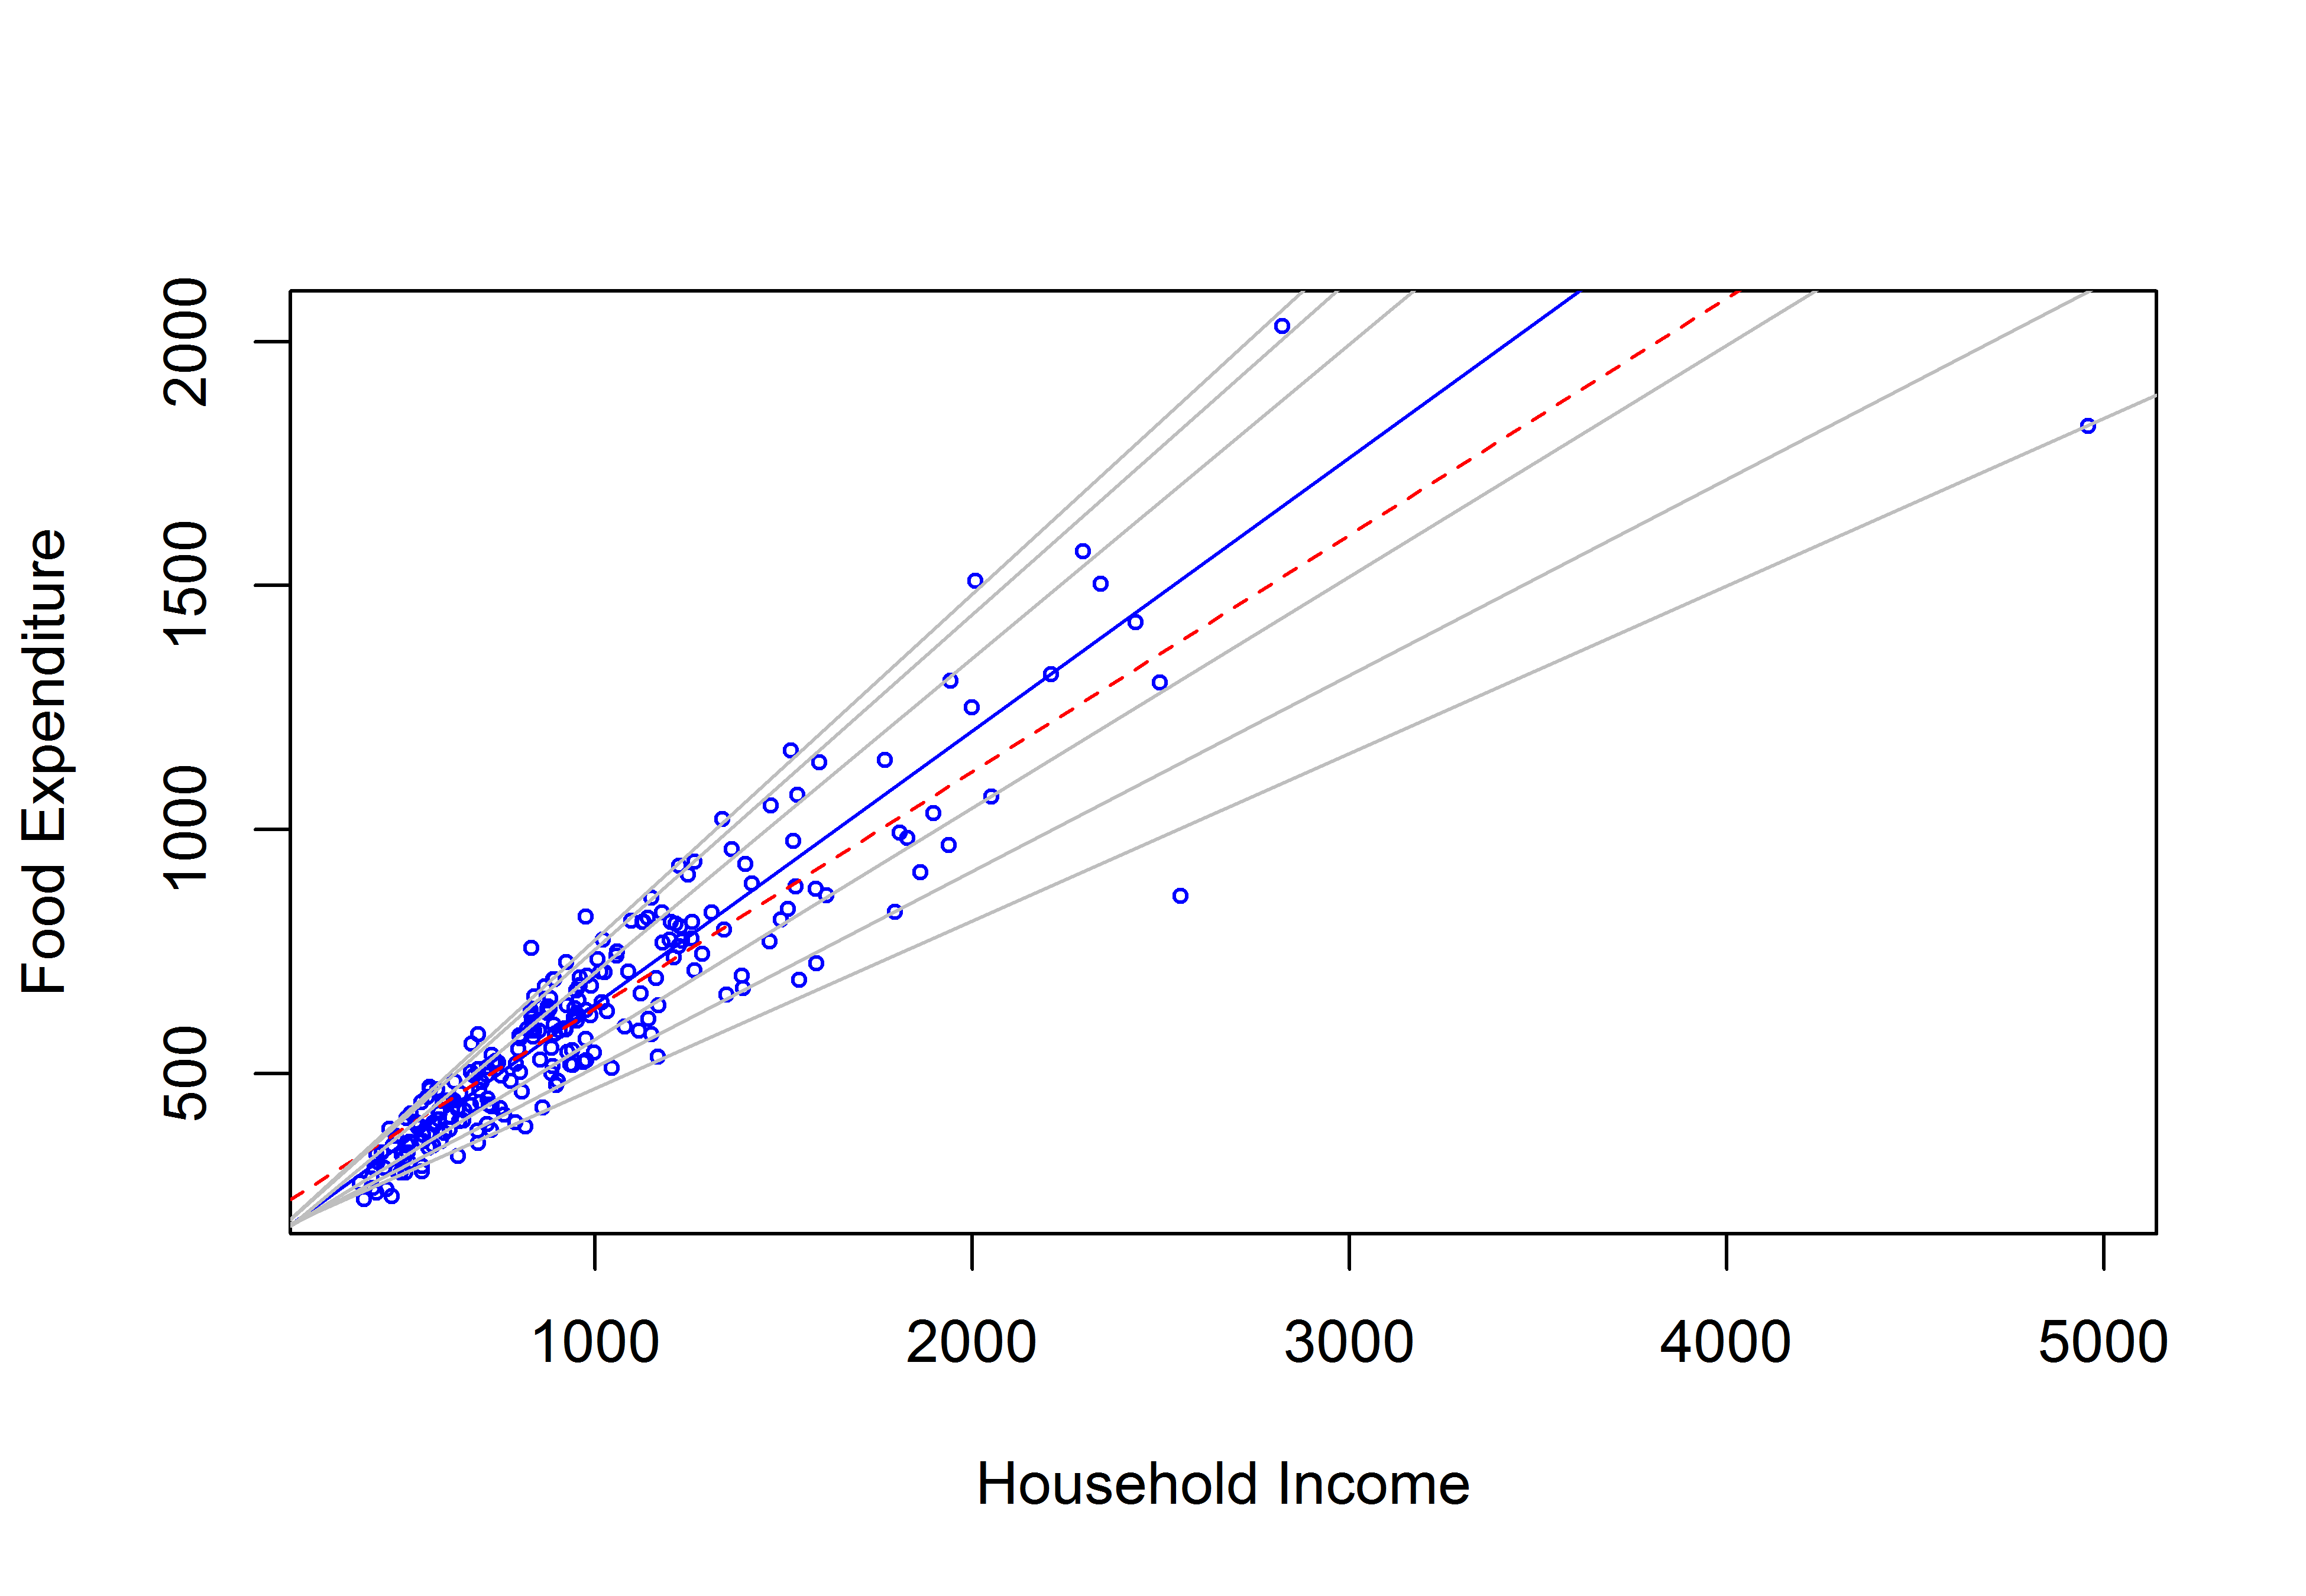
\includegraphics[width=0.7\linewidth]{images/engel-1} 

}

\caption{Comparação de modelos de regressão para média (em vermelho) e para a mediana (em azul).}\label{fig:engel}
\end{figure}

Na figura \ref{fig:engel} as retas cinzas são as regressões para os
quantis de 5\%, 10\%, 25\%, 75\%, 90\% e 95\%.

Também é possível a transformação de variáveis nos modelos de regressão
quantílica, assim como fazemos nos modelos de regressão à média. O
modelo de regressão linear para a média apresentado é heteroscedástico,
como o próprio gráfico da figura \ref{fig:engel} demonstra. Nestes
casos, é usual proceder com a transformação dos dados. Desta maneira,
foi elaborada a figura \ref{fig:engellog}, reproduzida da vinheta
(\protect\hyperlink{ref-quantregvignette}{2018}\protect\hyperlink{ref-quantregvignette}{a},
p. 11) do pacote \pkg{quantreg}
(\protect\hyperlink{ref-quantreg}{2018}\protect\hyperlink{ref-quantreg}{b})
do software estatístico \proglang{R} (\protect\hyperlink{ref-R}{2017}),
que nos mostra o modelo das variáveis em escala \emph{log}.

\begin{figure}[H]

{\centering 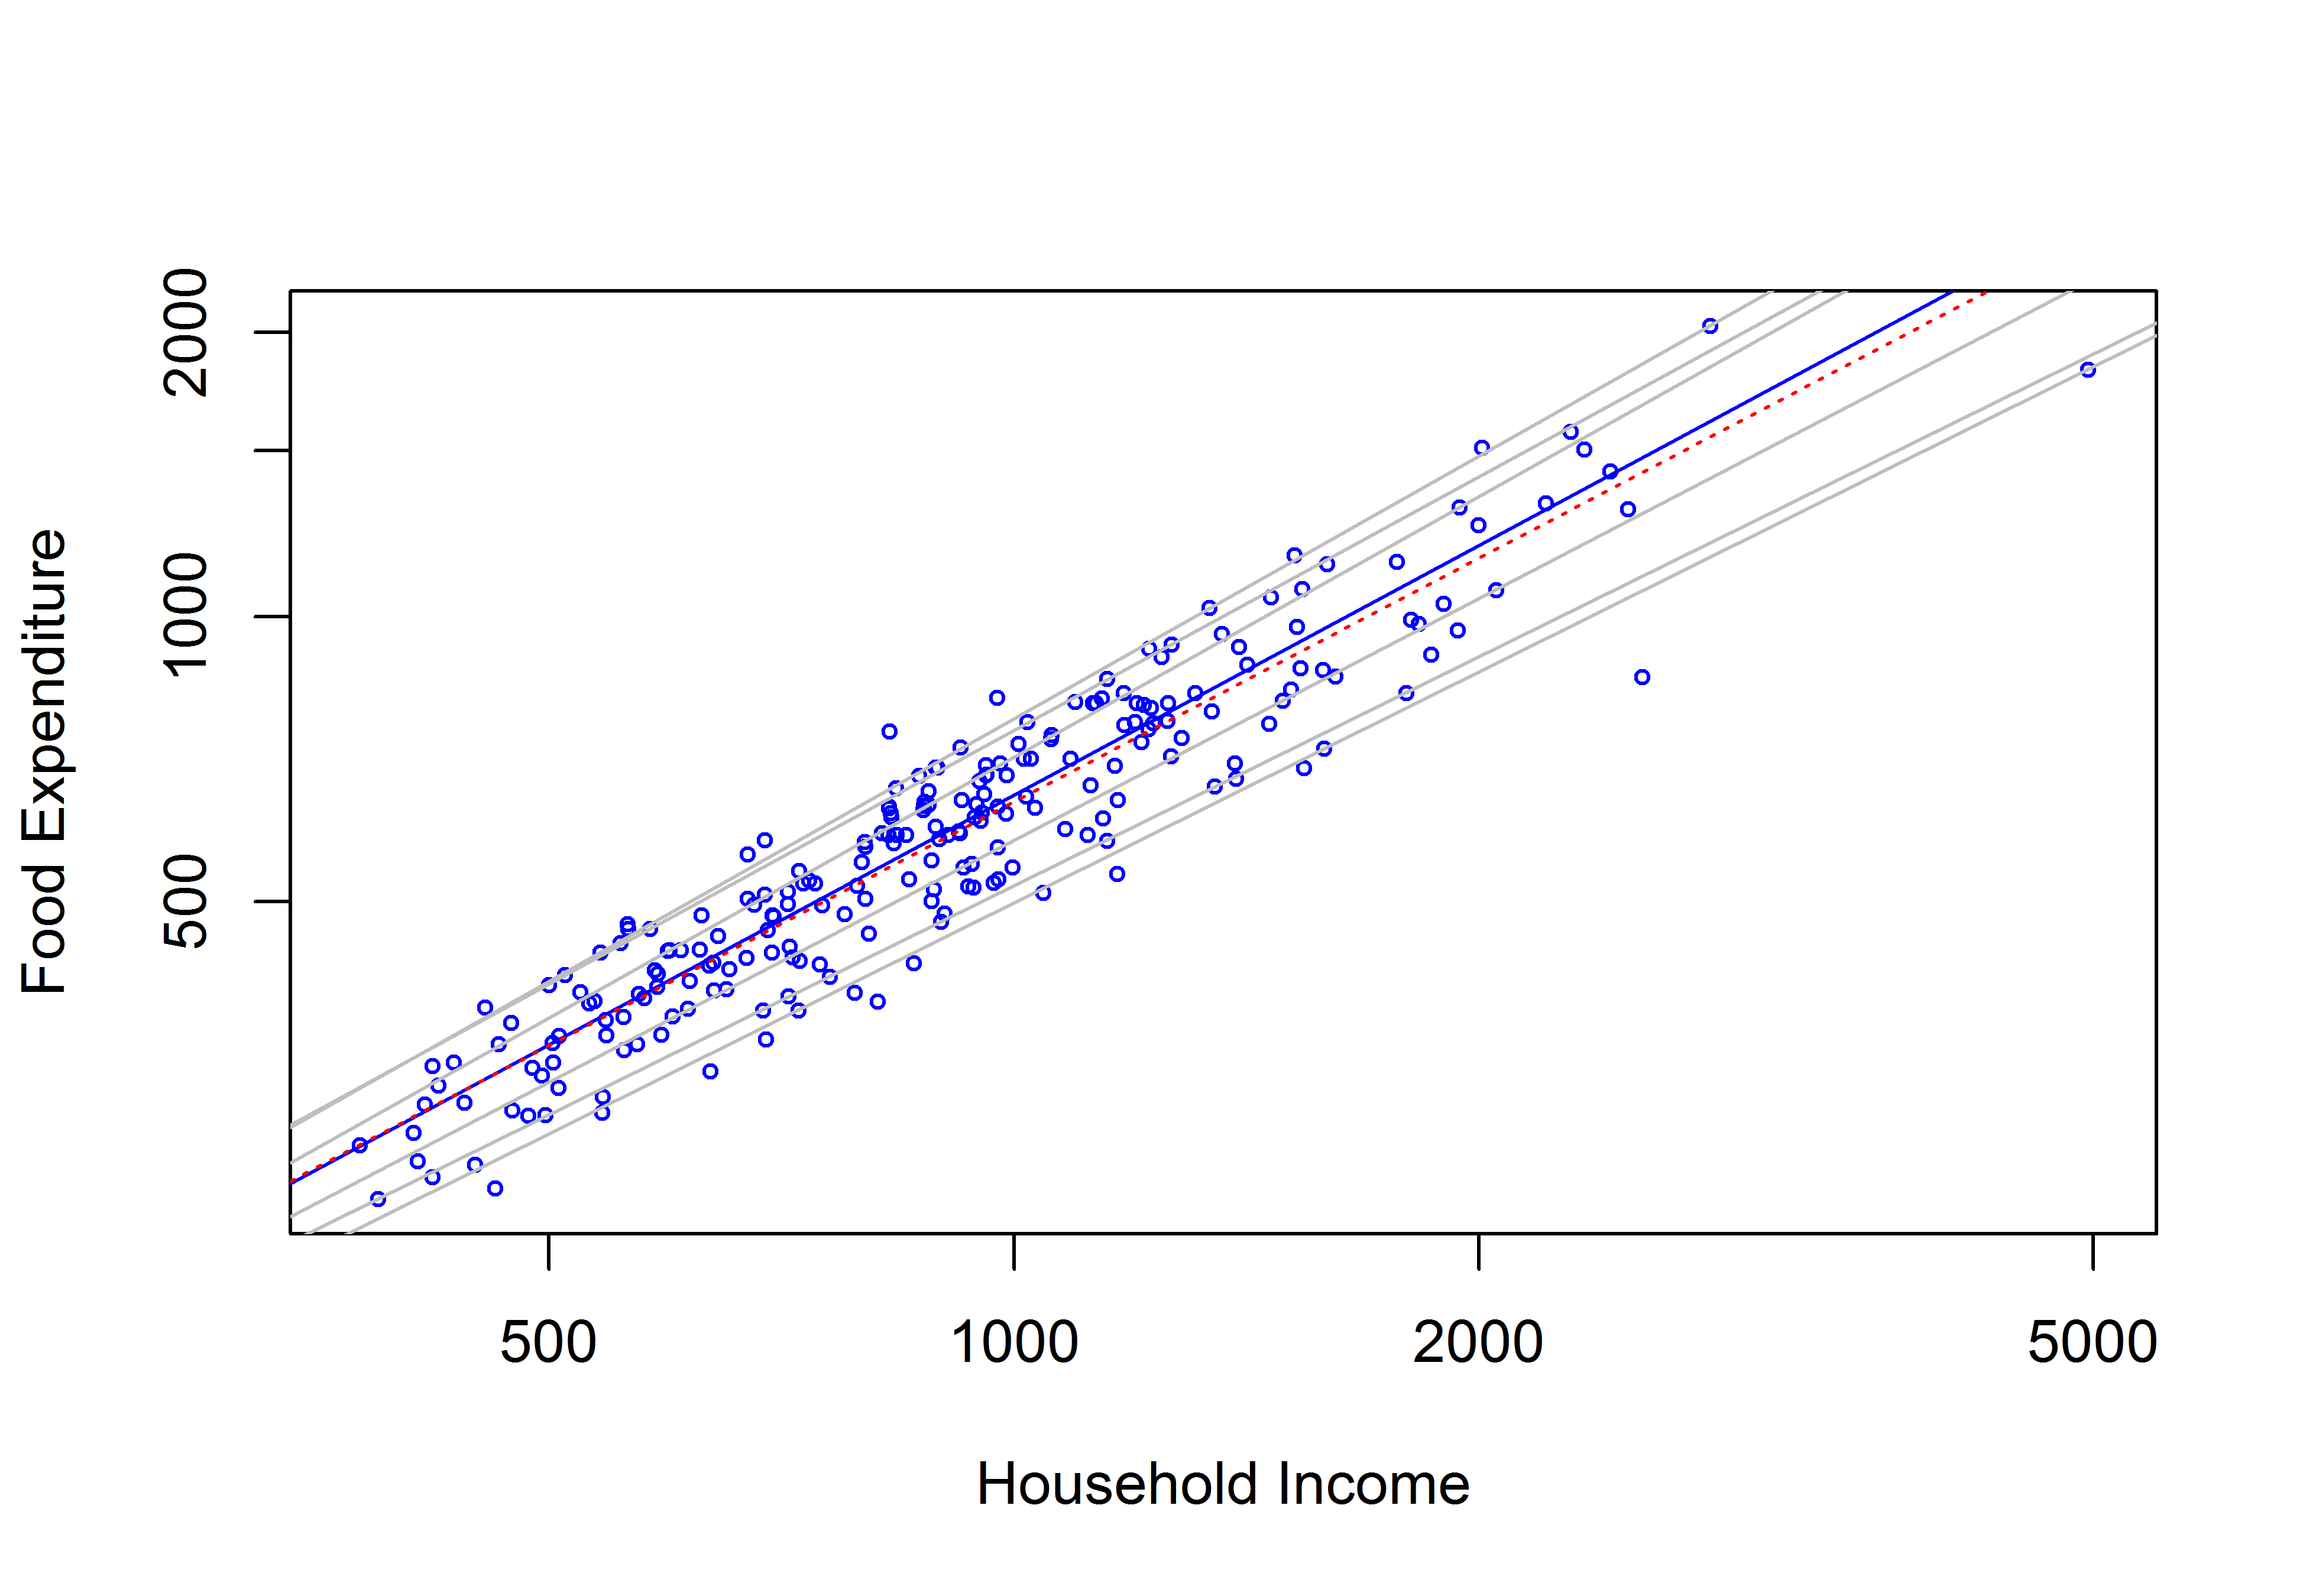
\includegraphics[width=0.7\linewidth]{images/engellog-1} 

}

\caption{Comparação de modelos de regressão para média (em vermelho) e para a mediana (em azul) em escala transformada (log).}\label{fig:engellog}
\end{figure}

Como esperado, a heteroscedasticidade do modelo desapareceu com a
transformação dos dados.

\subsection{O problema da retransformação das
variáveis}\label{o-problema-da-retransformacao-das-variaveis}

Segundo (SHEN; ZHU, \protect\hyperlink{ref-shen}{2008}, p. 552), modelos
lineares lognormais tem muitas aplicações e muitas vezes é de interesse
prever a variável resposta ou estimar a média da variável resposta na
escala original para um novo conjunto de covariantes.

Segundo Shen e Zhu(\protect\hyperlink{ref-shen}{2008}, p. 552), se
\(Z = (Z_1,\cdots, Z_n)^T\) é o vetor variável resposta de distribuição
lognormal e \(x_i = (1, x_{i1}, \cdots, x_{ip})^T\) é o vetor dos
covariantes para a observação \(i\), um modelo linear log-normal assume
a seguinte forma:

\[Y = log(Z) = X\beta + \epsilon\]

onde \(X = (x_1, \cdots, x_n)^T\),
\(\beta = (\beta_0, \beta_1, \cdots, \beta_p)^T\), e
\(\epsilon = (\epsilon_1, \cdots, \epsilon_n)^T\) com
\(\epsilon_i \sim N(0, \sigma^2)\) i.i.d.(\emph{identically
independently distributed}) (SHEN; ZHU,
\protect\hyperlink{ref-shen}{2008}, pp. 552--553).

\begin{quote}
Em muitos casos, para um novo conjunto de covariantes \(x_0\), pode-se
estar interessado em prever a variável resposta em sua escala original:

\[Z_0 = e^{x_o^T\beta + \epsilon_0}\]

ou estimar a média condicional da variável resposta:

\[\mu(x_0)=E[Z_0|x_o] = e^{x_o^T\beta + \frac{1}{2}\sigma^2}\]
\end{quote}

De acordo com Shen e Zhu(\protect\hyperlink{ref-shen}{2008}, p. 553), se
\(\beta\) e \(\sigma^2\) são ambos conhecidos, então é fácil demonstrar
que o melhor estimador de \(Z_0\) é de fato \(\mu(x_0)\). Contudo, na
prática, ambos \(\beta\) e \(\sigma^2\) são desconhecidos e precisam ser
estimados para a obtenção de \(\mu(x_0)\).

Segundo Shen e Zhu (\protect\hyperlink{ref-shen}{2008}, p. 552), existem
na literatura diversos estimadores baseados em diversos métodos
inferenciais, como \textbf{ML} (\emph{Maximum Likelihood Estimator}),
\textbf{REML} (\emph{Restricted ML Estimator}), \textbf{UMVU}
(\emph{Uniformly Minimum Variance Unbiased Estimator}), além de um
estimador \textbf{REML} com viés corrigido.

Na prática, estes estimadores pertencem a uma classe de estimadores
definida na expressão abaixo:

\[\begin{Bmatrix}
\hat{\mu_c}(x_0):\hat{\mu_c}(x_0) = exp(x_0^T\hat{\beta} + cRSS/2), c = \frac{1}{n-a}, a<n
\end{Bmatrix}\]

Shen e Zhu(\protect\hyperlink{ref-shen}{2008}) então propõem dois novos
estimadores baseados na minimização do erro médio quadrático assintótico
(\(MM\)) e do viés assintótico (\(MB\)).

De maneira que a diferença entre os estimadores supra-citados pode ser
resumida ao parâmetro \(a\):

\(a_{ML} = 0\)

\(a_{REML} = p+1\)

\(a_{MM} = p - 1 - 3nv_0 - 3RSS/(2m)\)

\(a_{MB} = p + 1 - nv_0 - RSS/(2m)\)

\subsubsection{Estimadores
não-paramétricos}\label{estimadores-nao-parametricos}

De acordo com Duan (\protect\hyperlink{ref-Duan}{1983}, p. 606), o Valor
Esperado \(E\) de uma variável resposta \(Y\) que tenha sido
transformada em valores \(\eta\) durante a regressão linear por uma
função \(g(Y)\) \textbf{não-linear} não é igual ao valor da simples
retransformação da variável transforma pela sua função inversa
\(h(\eta) = g^{-1}(Y)\). Em outros termos (DUAN,
\protect\hyperlink{ref-Duan}{1983}, p. 606):

\[E[Y_0] = E[h(x_0\beta + \epsilon)] \ne h(x_o\beta)\]

Reparar que o termo de erro faz parte da composição do valor esperado da
variável de regressão. Em uma regressão linear clássica, sem
transformação, \(E[\epsilon] = 0\), então \(E[Y_0] = E[x_0\beta]\).

Numa regressão log-linear, ou seja, uma regressão linear com o logaritmo
da variável dependente (\(h(\eta) = g^{-1}(\eta) = exp(\eta)\)), para
efetuar apropriadamente a retransformação das estimativas de volta a sua
escala original, precisa-se ter em conta a desigualdade mencionada na
seção \ref{esperanca-matematica-ou-valor-esperado}.

Segundo (MANNING; MULLAHY, \protect\hyperlink{ref-NBERt0246}{1999}),
quando ajustamos o logaritmo natural de uma variável \(Y\) contra outra
variável \(X\) através da seguinte equação de regressão:

\[ln(Y) = \beta_0 + \beta_1X + \epsilon\]

Se o erro \(\epsilon\) é normalmente distribuído, com média zero e
desvio padrão \(\sigma^2\), ou seja, se
\(\epsilon \sim N(0, \sigma^2)\), então (DUAN,
\protect\hyperlink{ref-Duan}{1983}, p. 606; MANNING; MULLAHY,
\protect\hyperlink{ref-NBERt0246}{1999}, p. 6):

\[E[Y|X] = e^{\beta_0 + \beta_1X} \cdot E[e^\epsilon] \ne e^{\beta_0 + \beta_1X}\]

Embora o valor esperado dos resíduos \(\epsilon\) seja igual a zero, ele
está submetido a uma transformação não linear, de maneira que não
podemos afirmar que \(E[e^\epsilon] = 1\) (como vimos na seção
\ref{desigualdade-de-jensen}, \(E[exp(x)] > exp[E(x)]\)). Desta maneira,
o estimador abaixo, chamado em (SHEN; ZHU,
\protect\hyperlink{ref-shen}{2008}, p. 554) de \emph{naive
back-transform estimator}, ou simplesmente \textbf{BT} não é consistente
e é enviesado, tendo viés multiplicativo de valor assintótico igual a
\(e^{-\sigma^2/2}\):

\[E[Y|X] = e^{\beta_0 + \beta_1X}\]

Segundo (SHEN; ZHU, \protect\hyperlink{ref-shen}{2008}, p. 554), ainda,
o valor de \(e^{-\sigma^2/2}\) é sempre menor do que 1(SHEN; ZHU,
\protect\hyperlink{ref-shen}{2008}, p. 554).

\begin{quote}
As a result, the BT estimator underestimates \(\mu(x_0)\), and the bias
is large when \(\sigma^2\) is large. In our study, it appears that the
BT estimator performs much worse than the other
estimators{[}\ldots{}{]}Actually, the BT estimator is more suitable for
estimating the median of Z0, which is \(exp(x_0^T\beta)\) in this case.
\end{quote}

Porém se o termo de erro \(\epsilon\) é normalmente distribuído
\(N(0,\sigma^2)\), então um estimador não-enviesado para o valor
esperado \(E[Y]\), de acordo com DUAN
(\protect\hyperlink{ref-Duan}{1983}), assume a forma vista na equação
abaixo(DUAN, \protect\hyperlink{ref-Duan}{1983}, p. 606; MANNING;
MULLAHY, \protect\hyperlink{ref-NBERt0246}{1999}, p. 2 e 6):

\[E[Y] = e^{\beta_0 + \beta_1X} \cdot e^{\frac{1}{2}\sigma^2}\]

Cabe salientar, segundo (MANNING; MULLAHY,
\protect\hyperlink{ref-NBERt0246}{1999}, p. 6), que se o termo de erro
não for i.i.d (independente e identicamente distribuído), mas for
homoscedástico, então:

\[E[Y|X]=s \times e^{X_0\beta}\] onde \(s = E[e^\epsilon]\).

De qualquer maneira, o valor esperado de \(Y\) é proporcional à
exponencial da previsão na escala log.

DUAN (\protect\hyperlink{ref-Duan}{1983}) apresenta então um estimador
não-paramétrico (\emph{smearing estimate}), independente da função de
transformação \(h(\eta)\) e da distribuição dos erros \(F(\epsilon)\),
tal que:

\[\hat{E}[Y_0] = \int h(x_0\hat{\beta} + \epsilon)d\hat{F}_n(\epsilon) = \frac{1}{n}\sum_{i = 1}^{n}h(x_0\hat{\beta}+\hat{\epsilon_i})\]

\subsubsection{Modelos
Heteroscedásticos}\label{modelos-heteroscedasticos}

Modelos heteroscedásticos não são raros, especialmente no caso de
variáveis envolvendo valores em moeda, sendo muito comum em modelos
econométricos. Em sua essência, são heteroscedásticos aqueles modelos
lineares cujo termo de erro não pode ser considerado totalmente
independente, ou seja, existe alguma função (linear ou não), tal que
\(E[e^\epsilon] = f(x)\), de modo que:

\[log(E[Y|X]) = X\beta + log(f(x))\]

É desnecessário dizer que, para estes modelos o estimador para a média é
diferente de
\(E[Y] = e^{\beta_0 + \beta_1X} \cdot e^{\frac{1}{2}\sigma^2}\), haja
vista que \(\sigma^2\) não é mais um escalar, mas uma função.

Existem diversas maneiras de se contornar este problema. Por exemplo,
através da eliminação do viés através da utilização de uma função que
modele a variância \(\sigma^2(X)\), ou através do estimador
sanduíche\footnote{ver
  \href{https://matloff.wordpress.com/2015/09/18/can-you-say-heteroscedasticity-3-times-fast/}{link}}.

Cabe ainda salientar que, para os modelos heteroscedásticos, não apenas
os erros estão comprometidos, mas também os intervalos de confiança.

\subsection{Validação Cruzada}\label{validacao-cruzada}

Validação Cruzada ou \emph{cross-validation} é uma técnica estatística
que pode ser utilizada de diversas maneiras e consistem em dividir um
conjunto de dados em duas partições distintas, chamados de partição de
treino (\emph{training set}) e partição de teste(\emph{test set}),
utilizadas para o ajuste do modelo e para a previsão da variável
dependente, respectivamente. Os dados previstos na partição de teste são
então comparados aos valores observados.

Neste artigo efetuaremos a validação-cruzada utilizando o procedimento
chamado de \emph{delete-one procedure}, em que se retira apenas um dado
do conjunto de dados, ajusta-se um modelo e então utiliza-se este modelo
para prever o valor da variável dependente para o dado retirado (SHEN;
ZHU, \protect\hyperlink{ref-shen}{2008}, p. 564).

Para cada observação então calcula-se o seu erro quadrático
(\((Y_i - \hat{Y}_i)^2\)), utilizado para o cálculo da estatística RMSPE
(erro de previsão médio quadrático, ou \emph{root mean squared
prediction error}), conforme expressão a seguir (SHEN; ZHU,
\protect\hyperlink{ref-shen}{2008}, p. 564):

\[RMSPE = (\frac{1}{n}\sum_{i = 1}^{n}(Y_i - \hat{Y}_i)^2)^{1/2}\]

\section{ESTUDO DE CASO}\label{estudo-de-caso}

Com o fim de averiguar qual estimador melhor se adequa ao procedimento
de retransformação de variáveis, aplicar-se-á um comparativo entre os
estimadores média, moda e mediana, através do uso da estatística RMSPE.

\subsection{Dados}\label{dados}

Neste estudo comparamos a precisão de diversos tipos de modelos
estatísticos (regressão linear, regressão não-linear e modelo linear
generalizado) sobre os dados disponíveis em Hochheim
(\protect\hyperlink{ref-hochheim}{2015}, pp. 21--22).

Os coeficientes do modelo utilizado em HOCHHEIM
(\protect\hyperlink{ref-hochheim}{2015}), assim como suas estatísticas
básicas podem ser visualizados na tabela \ref{tab:fit}.

\subsection{Cálculo do RMSPE}\label{calculo-do-rmspe}

\subsubsection{Regressão linear
ordinária}\label{regressao-linear-ordinaria}

Para o cálculo do RMSPE foi utilizado como referência o modelo proposto
por Hochheim (\protect\hyperlink{ref-hochheim}{2015}, p. 29), ou seja,
foram utilizadas as mesmas transformações de variáveis utilizadas no
modelo proposto. Os valores dos \(\beta_i\) são calculados a cada passo.

Os valores encontrados para o erro de predição médio quadrático para
cada estimador foram: \textbf{R\$203.939,11} para a média,
\textbf{R\$204.006,84} para a mediana e \textbf{R\$205.537,36} para a
moda.

Como esperado, o RMSPE foi menor para a média, e maior para a moda. O
que comprova a teoria, já que o \emph{naive estimator} é enviesado com
viés conhecido de \(-\sigma^2/2\), logo a moda possui viés de
\(-1,5\sigma^2\).

Os valores ajustados com os estimadores da moda, média e mediana podem
ser vistos na tabela \ref{tab:tabela}:

\subsection{Cálculo do erro médio
absoluto}\label{calculo-do-erro-medio-absoluto}

Assim como a regressão linear é uma minimização do erro médio
quadrático, a regressão à mediana leva a minimização do erro médio
absoluto.

Para verificarmos isto, com um modelo de regressão à mediana,
calcularemos o RMAPE (\emph{root mean absolute prediction error}) e o
RMSPE (\emph{root mean squared prediction error}) para as estimativas
obtidas com este modelo.

\subsubsection{Regressão quantílica à
mediana}\label{regressao-quantilica-a-mediana}

O modelo de regressão quantílica com quantil \(\tau = 0.5\), ou seja, o
modelo de regressão à mediana, para os mesmos dados supra-mencionados
está resumido na tabela \ref{tab:fit}.

\begin{table}[!htbp] \centering 
  \caption{Comparação entre os coeficientes de regressão linear e regressão quantílica} 
  \label{tab:fit} 
\begin{tabular}{@{\extracolsep{5pt}}lcc} 
\\[-1.8ex]\hline 
\hline \\[-1.8ex] 
 & \multicolumn{2}{c}{\textit{Dependent variable:}} \\ 
\cline{2-3} 
\\[-1.8ex] & \multicolumn{2}{c}{log(valor)} \\ 
\\[-1.8ex] & \textit{OLS} & \textit{quantile} \\ 
 & \textit{} & \textit{regression} \\ 
\\[-1.8ex] & (1) & (2)\\ 
\hline \\[-1.8ex] 
 area\_total & 0.001 & 0.002 \\ 
  & (0.001, 0.002) & (0.0003, 0.003) \\ 
  & t = 5.113 & t = 2.300 \\ 
  & p = 0.00001$^{***}$ & p = 0.027$^{**}$ \\ 
  & & \\ 
 quartos & 0.164 & 0.162 \\ 
  & (0.094, 0.233) & (0.078, 0.245) \\ 
  & t = 4.626 & t = 3.788 \\ 
  & p = 0.00004$^{***}$ & p = 0.0005$^{***}$ \\ 
  & & \\ 
 suites & 0.061 & 0.080 \\ 
  & ($-$0.005, 0.127) & ($-$0.012, 0.171) \\ 
  & t = 1.810 & t = 1.712 \\ 
  & p = 0.078$^{*}$ & p = 0.095$^{*}$ \\ 
  & & \\ 
 garagens & 0.209 & 0.152 \\ 
  & (0.143, 0.274) & (0.034, 0.271) \\ 
  & t = 6.247 & t = 2.520 \\ 
  & p = 0.00000$^{***}$ & p = 0.016$^{**}$ \\ 
  & & \\ 
 log(dist\_b\_mar) & $-$0.141 & $-$0.146 \\ 
  & ($-$0.194, $-$0.087) & ($-$0.244, $-$0.047) \\ 
  & t = $-$5.174 & t = $-$2.904 \\ 
  & p = 0.00001$^{***}$ & p = 0.006$^{***}$ \\ 
  & & \\ 
 I(padrao$\hat{\mkern6mu}$-1) & $-$0.563 & $-$0.459 \\ 
  & ($-$0.769, $-$0.357) & ($-$0.751, $-$0.166) \\ 
  & t = $-$5.360 & t = $-$3.070 \\ 
  & p = 0.00001$^{***}$ & p = 0.004$^{***}$ \\ 
  & & \\ 
 Constant & 13.564 & 13.574 \\ 
  & (13.112, 14.016) & (12.850, 14.298) \\ 
  & t = 58.847 & t = 36.732 \\ 
  & p = 0.000$^{***}$ & p = 0.000$^{***}$ \\ 
  & & \\ 
\hline \\[-1.8ex] 
Observations & 48 & 50 \\ 
R$^{2}$ & 0.956 &  \\ 
Adjusted R$^{2}$ & 0.950 &  \\ 
Akaike Inf. Crit. & $-$46.813 & $-$38.299 \\ 
Residual Std. Error & 0.136 (df = 41) &  \\ 
F Statistic & 148.921$^{***}$ (df = 6; 41) &  \\ 
\hline 
\hline \\[-1.8ex] 
\textit{Note:}  & \multicolumn{2}{r}{$^{*}$p$<$0.1; $^{**}$p$<$0.05; $^{***}$p$<$0.01} \\ 
\end{tabular} 
\end{table}

De posse do modelo para a regressão quantílica, fazemos a previsão para
a mediana da variável \texttt{valor} na escala original da mesma maneira
que a fizemos para a regressão linear, ou seja, apenas aplicamos a
função inversa à variável transformada (\(valor = exp(log(\hat{Y}))\)).
Os valores podem ser vistos na tabela \ref{tab:tabela}.

\rowcolors{2}{gray!6}{white}

\begin{table}

\caption{\label{tab:tabela}Valores ajustados para os dados pelos estimadores}
\centering
\begin{tabular}[t]{lrrrrr}
\hiderowcolors
\toprule
\multicolumn{1}{c}{ } & \multicolumn{1}{c}{Dados} & \multicolumn{3}{c}{Regressão Linear} & \multicolumn{1}{c}{Regressão Quantílica} \\
\cmidrule(l{2pt}r{2pt}){2-2} \cmidrule(l{2pt}r{2pt}){3-5} \cmidrule(l{2pt}r{2pt}){6-6}
  & Y & Média & Mediana & Moda & Mediana.1\\
\midrule
\showrowcolors
AP\_1 & 1.060.000 & 1.029.765 & 1.020.713 & 1.002.846 & 996.289\\
AP\_2 & 510.000 & 628.132 & 622.610 & 611.712 & 639.691\\
AP\_3 & 780.000 & 855.052 & 847.535 & 832.700 & 831.259\\
AP\_4 & 550.000 & 736.956 & 730.478 & 717.691 & 744.529\\
AP\_5 & 850.000 & 1.011.300 & 1.002.410 & 984.863 & 1.012.810\\
\addlinespace
AP\_6 & 300.000 & 358.594 & 355.441 & 349.220 & 366.587\\
AP\_7 & 750.000 & 724.106 & 717.741 & 705.177 & 688.216\\
AP\_8 & 650.000 & 657.475 & 651.695 & 640.288 & 670.429\\
AP\_9 & 620.000 & 658.389 & 652.601 & 641.177 & 668.602\\
AP\_10 & 740.000 & 662.002 & 656.182 & 644.696 & 671.303\\
\addlinespace
AP\_11 & 770.000 & 818.933 & 811.734 & 797.525 & 796.637\\
AP\_12 & 680.000 & 702.573 & 696.397 & 684.207 & 730.751\\
AP\_13 & 850.000 & 681.544 & 675.553 & 663.728 & 703.913\\
AP\_14 & 420.000 & 551.781 & 546.931 & 537.357 & 602.931\\
AP\_15 & 547.000 & 673.810 & 667.887 & 656.196 & 671.661\\
\addlinespace
AP\_16 & 1.600.000 & 1.413.047 & 1.400.625 & 1.376.108 & 1.380.730\\
AP\_17 & 1.320.000 & 1.115.664 & 1.105.857 & 1.086.499 & 1.089.621\\
AP\_18 & 615.000 & 645.338 & 639.665 & 628.468 & 656.846\\
AP\_19 & 705.000 & 722.736 & 716.383 & 703.843 & 683.668\\
AP\_20 & 418.000 & 435.824 & 431.993 & 424.431 & 424.671\\
\addlinespace
AP\_21 & 270.000 & 243.440 & 241.300 & 237.077 & 269.827\\
AP\_22 & 418.000 & 485.426 & 481.159 & 472.736 & 482.432\\
AP\_23 & 650.000 & 630.016 & 624.478 & 613.547 & 617.157\\
AP\_24 & 700.000 & 774.614 & 767.805 & 754.365 & 732.197\\
AP\_25 & 680.000 & 729.864 & 723.448 & 710.784 & 688.216\\
\addlinespace
AP\_26 & 420.000 & 350.336 & 347.256 & 341.178 & 375.896\\
AP\_27 & 195.000 & 229.411 & 227.394 & 223.414 & 245.742\\
AP\_28 & 290.000 & 279.686 & 277.228 & 272.375 & 290.168\\
AP\_29 & 272.000 & 246.194 & 244.030 & 239.758 & 256.602\\
AP\_30 & 430.000 & 399.634 & 396.121 & 389.187 & 419.334\\
\addlinespace
AP\_31 & 895.000 & 615.032 & 609.625 & 598.954 & 617.838\\
AP\_32 & 450.000 & 454.828 & 450.830 & 442.938 & 446.205\\
AP\_33 & 1.950.000 & 1.474.903 & 1.461.938 & 1.436.347 & 1.377.397\\
AP\_34 & 2.150.000 & 2.597.848 & 2.575.011 & 2.529.937 & 2.489.511\\
AP\_35 & 940.000 & 969.142 & 960.623 & 943.808 & 949.471\\
\addlinespace
AP\_36 & 1.400.000 & 1.334.839 & 1.323.105 & 1.299.945 & 1.367.813\\
AP\_37 & 1.090.000 & 1.002.811 & 993.996 & 976.596 & 874.599\\
AP\_38 & 1.272.000 & 999.341 & 990.556 & 973.217 & 995.271\\
AP\_39 & 2.800.000 & 1.921.706 & 1.904.812 & 1.871.470 & 1.850.329\\
AP\_40 & 1.796.000 & 2.075.621 & 2.057.374 & 2.021.361 & 2.001.997\\
\addlinespace
AP\_41 & 1.400.000 & 1.398.114 & 1.385.824 & 1.361.566 & 1.402.080\\
AP\_42 & 3.000.000 & 3.306.637 & 3.277.569 & 3.220.197 & 3.153.592\\
AP\_43 & 1.200.000 & 1.062.442 & 1.053.103 & 1.034.669 & 1.058.339\\
AP\_44 & 800.000 & 646.536 & 640.853 & 629.635 & 681.151\\
AP\_45 & 950.000 & 668.014 & 662.142 & 650.551 & 685.574\\
\addlinespace
AP\_46 & 2.061.000 & 2.267.978 & 2.248.041 & 2.208.690 & 2.183.863\\
AP\_47 & 1.326.000 & 1.575.944 & 1.562.090 & 1.534.746 & 1.538.481\\
AP\_48 & 850.000 & 776.375 & 769.550 & 756.079 & 748.939\\
AP\_49 & 1.650.000 & 1.509.488 & 1.496.218 & 1.470.028 & 1.439.387\\
AP\_50 & 650.000 & 834.750 & 827.412 & 812.929 & 854.382\\
\bottomrule
\multicolumn{6}{l}{\textsuperscript{1} Estimada pela regressão à mediana.}\\
\end{tabular}
\end{table}

\rowcolors{2}{white}{white}

O valor de RMAPE para a regressão à mediana é de R\$131.842,83, enquanto
o valor do RMSPE é de R\$208.063,86.

É fácil demonstrar que estes valores são bem diferentes dois obtidos
pelas estimativas da regressão linear clássica (regressão à média). Para
a estimativa pela mediana na regressão linear, o erro médio absoluto
seria de R\$ 133.234,00, bem superior ao erro médio absoluto obtido pela
regressão à mediana.

Já para o RMSPE, o valor obtido na regressão linear é menor, qualquer
que seja a estimativa, pela moda, média ou mediana.

Ou seja, o modelo de regressão linear minimizou o RMSPE e o modelo de
regressão quantílica minimizou o RMAPE, conforme esperado.

\section{CONCLUSÃO}\label{conclusao}

Como vimos na seção \ref{revisao-bibliografica}, o método clássico de
regressão linear é uma minimização do erro médio quadrático de predição
e a função de regressão \(\hat{m}_{Y;X}\) é uma equação para a
\emph{média} da população \(Y\) dado \(X\), seja ela uma função de outra
variável ou não. Considerando que são satisfeitas as hipóteses da
regressão linear clássica, o melhor estimador para o valor será o da
avaliação pela média, haja vista que, por definição, a regressão linear
é uma função para a média.

Ora, claro está, de acordo com todos os trabalhos citados, inclusive
GIANNAKOS; LEÃO (\protect\hyperlink{ref-giannakos}{1996}), que o valor
esperado da variável é a média. A regressão linear com o método dos
mínimos quadrados é uma regressão para a média. Isto posto, como então
avaliar o valor da variável original? Porque na área de avaliações não
temos interesse na previsão da variável \(W = log(Y)\), mas sim na
variável \(Y\), ou seja, estamos interessados nos valores da variável
original, não nos valores da variável transformada. Está claro que
deve-se proceder a retransformação da variável \(W\) na variável
original, mas para isso é preciso utilizar o método correto.

Esperamos ter demonstrado com este artigo que a retransformação adequada
da variável de regressão linear é a estimativa pela média, que é o seu
Valor Esperado, que pode ser calculado através de qualquer dos
estimadores supra-citados, sem com isso adulterar a equação de
regressão, muito pelo contrário, reafirmando-a.

Não pretendemos, com isto, impor quer seja a média ou a mediana a melhor
estimativa. Em vários campos, a mediana tem sido adotada como melhor
estimativa, por sua propriedade de estar menos vulnerável a presença de
\emph{outliers}, como ocorre com a média.

No entanto, se pretende-se efetuar uma avaliação pela mediana,
entendemos que a melhor opção seria a utilização da regressão
quantílica, para o quantil de 50\% (obviamente), e não a utilização da
retransformação inadequada da equação de regressão linear, que
destina-se a estimar a média.

Em relação à moda como estimativa de medida central, consideramos que
esta se trata mais de uma curiosidade do que uma estimativa de fato: o
que significa a moda de uma população de apartamentos em uma determinada
cidade? A moda encontraria-se, provavelmente, nos valores dos
apartamentos de 2 e 3 quartos, com uma ou duas vagas de garagem. Mas
qual a utilidade disto quando o que se pretende avaliar, por exemplo, é
o valor de um apartamento de 4 ou 5 quartos e 4 ou 5 vagas de garagem,
ou ainda de se avaliar um apartamento com um quarto e sem vaga de
garagem? Assim como os apartamento citados estão ``fora de moda'',
também estarão os seu valores. Contudo, estes estarão em consonância com
a média ou com a mediana do mercado, dados as suas características, a
depender da configuração deste.

Em outras palavras, um modelo de regressão linear é uma média
\emph{condicional} da variável resposta (ver
\protect\hyperlink{regressao-linear}{Regressão Linear}). Ou seja,
pretende-se saber o valor médio de um imóvel \emph{dado que} ele possui
as seguintes características\ldots{}E estas características podem estar
\emph{na moda} ou fora dela.

\section*{REFERÊNCIAS}\label{referencias}
\addcontentsline{toc}{section}{REFERÊNCIAS}

\hypertarget{refs}{}
\hypertarget{ref-NBR1465302}{}
ABNT. \textbf{NBR 14653-2: Avaliação de bens -- parte 2: Imóveis
urbanos}. Rio de Janeiro: Associação Brasileira de Normas Técnicas,
2011.

\hypertarget{ref-bennett}{}
BENNETT, H. Lecture note 4: Expectations (moments)., 2006. MIT.
Disponível em:
\textless{}\url{https://ocw.mit.edu/courses/economics/14-30-introduction-to-statistical-method-in-economics-spring-2006/lecture-notes/l4.pdf}\textgreater{}..

\hypertarget{ref-gkchesterton}{}
CHESTERTON, G. K. \textbf{Ortodoxia}. São Paulo: Mundo Cristão, 2008.

\hypertarget{ref-QR}{}
CRISTINA DAVINO, M. F.; VISTOCCO, D. \textbf{Quantile regression: Theory
and applications}. UK: Wiley, 2014.

\hypertarget{ref-Duan}{}
DUAN, N. Smearing estimate: A nonparametric retransformation method.
\textbf{Journal of the American Statistical Association}, v. 78, n. 383,
p. 605--610, 1983. Taylor \& Francis. Disponível em:
\textless{}\url{http://www.tandfonline.com/doi/abs/10.1080/01621459.1983.10478017}\textgreater{}..

\hypertarget{ref-giannakos}{}
GIANNAKOS, I. B. D. S.; LEÃO, M. L. Crítica à avaliação pela moda da
distribuição lognormal. In: VIII Congresso Brasileiro de Avaliações e
Perícias. \textbf{Anais\ldots{}}. p.267--278, 1996. Florianópolis:
COBREAP.

\hypertarget{ref-hochheim}{}
HOCHHEIM, N. \textbf{Engenharia de avaliações - módulo básico}.
Florianópolis: IBAPE - SC, 2015.

\hypertarget{ref-quantregvignette}{}
KOENKER, R. Quantile regression in R: A vignette., 2018a. Disponível em:
\textless{}\url{https://cran.r-project.org/web/packages/quantreg/vignettes/rq.pdf}\textgreater{}..

\hypertarget{ref-quantreg}{}
KOENKER, R. \textbf{Quantreg: Quantile regression}. 2018b.

\hypertarget{ref-koenker}{}
KOENKER, R.; HALLOCK, K. F. Quantile regression. \textbf{Journal of
Economic Perspectives}, v. 15, n. 4, p. 143--156, 2001.

\hypertarget{ref-NBERt0246}{}
MANNING, W. G.; MULLAHY, J. \textbf{Estimating log models: To transform
or not to transform?} Working Paper, National Bureau of Economic
Research, 1999.

\hypertarget{ref-matloff2009}{}
MATLOFF, N. S. \textbf{From Algorithms to Z-Scores: Probabilistic and
statistical modeling in computer science}. Davis, California: Orange
Grove Books, 2009.

\hypertarget{ref-R}{}
R CORE TEAM. \textbf{R: A language and environment for statistical
computing}. Vienna, Austria: R Foundation for Statistical Computing,
2017.

\hypertarget{ref-shen}{}
SHEN, H.; ZHU, Z. Efficient mean estimation in log-normal linear models.
\textbf{Journal of Statistical Planning and Inference}, v. 138, p.
552--567, 2008. Elsevier. Disponível em:
\textless{}\url{https://www.unc.edu/~haipeng/publication/emplnM1.pdf}\textgreater{}..


\end{document}
